\documentclass[12pt,a4paper]{article}
\usepackage[utf8]{inputenc}
\usepackage[T1]{fontenc}
\usepackage[portuguese]{babel}
\usepackage{graphicx}
\usepackage{float}
\usepackage{geometry}
\usepackage{amsmath}
\usepackage{booktabs}
\usepackage{enumitem}
\usepackage{xcolor}
\usepackage[hidelinks]{hyperref}
\geometry{a4paper, margin=2.5cm}
\setlist[itemize]{itemsep=2pt, topsep=4pt}

\newcommand{\graus}{$^\circ$}
\newcommand{\atencao}[1]{\textcolor{red!70!black}{\textbf{#1}}}

\title{\textbf{Análise dos Resultados: Modelo NARX, MPC Neural em Python, SIL no STM32 e Bancada do Aeropêndulo}}
\author{Felipe Eduardo Marcondes}
\date{\today}

\begin{document}

\maketitle

\begin{abstract}
Este documento analisa, em forma de tópicos, os principais resultados obtidos em cada etapa do projeto: (i) o modelo NARX polinomial identificado; (ii) o controle preditivo (NMPC) e sua aproximação por rede neural simulados em Python; (iii) a execução da rede embarcada no STM32 em \textit{Software-in-the-Loop} (SIL); e (iv) a validação na bancada física do aeropêndulo. Ao final, são apontadas inconsistências no relatório principal e melhorias sugeridas.
\end{abstract}

%==========================================================
\section{Modelo NARX identificado}
%==========================================================

\subsection{Configuração da identificação}
\begin{itemize}
    \item \textbf{Dados}: 6 ensaios de treino (multisseno, \textit{chirp} e APRBS) em \textbf{dois pontos de operação, 45\graus{} e 60\graus{}}; 3 ensaios de validação, todos em \textbf{45\graus{}}.
    \item \textbf{Pré-processamento}: descarte de 10\,s no início e 13\,s no final de cada ensaio, sem decimação ($T_s = 10$\,ms, 100\,Hz).
    \item \textbf{Dados em malha fechada} (PID de base): mantêm a planta estável e excitada, mas a entrada fica correlacionada com o ruído. Isso pode introduzir viés em estimadores de mínimos quadrados e deve ser citado como limitação.
    \item \textbf{Estrutura candidata}: $n_y = n_u = 15$ e grau polinomial $\ell = 2$, o que gera cerca de \textbf{496 regressores candidatos} (1 constante, 30 lineares e 465 quadráticos).
    \item \textbf{Seleção de estrutura}: \texttt{n\_components = 10}. O algoritmo FROLS (critério ERR) mantém apenas \textbf{10 termos}, resultando em um modelo bastante parcimonioso.
\end{itemize}

\subsection{Termos selecionados e interpretação física}

\begin{table}[H]
    \centering
    \caption{Termos e parâmetros do modelo NARX identificado.}
    \label{tab:narx}
    \begin{tabular}{@{}lrl@{}}
        \toprule
        \textbf{Termo} & \textbf{$\theta$} & \textbf{Interpretação} \\ \midrule
        $y(k-1)$          & $+1{,}4230$                & Dinâmica dominante (inércia) \\
        $y(k-2)$          & $-0{,}2120$                & Inércia / amortecimento (2ª ordem) \\
        $y(k-4)$          & $-0{,}1568$                & Amortecimento \\
        $y(k-10)$         & $-0{,}0944$                & Dinâmica lenta / memória longa \\
        $y(k-15)$         & $+0{,}0388$                & Memória longa (150\,ms) \\
        $y(k-1)^2$        & $+6{,}9\times10^{-6}$      & Não-linearidade estática (gravidade, $\sim\sin\theta$) \\
        $u(k-3)u(k-6)$    & $-9{,}3\times10^{-7}$      & Empuxo $\propto u^2$ \\
        $u(k-6)u(k-9)$    & $+1{,}77\times10^{-5}$     & Empuxo $\propto u^2$ (termo de entrada dominante) \\
        $u(k-3)u(k-15)$   & $+9{,}3\times10^{-6}$      & Empuxo $\propto u^2$ \\
        constante         & $-0{,}0059$                & \textit{Offset} (gravidade / zona morta do ESC) \\ \bottomrule
    \end{tabular}
\end{table}

\begin{itemize}
    \item \textbf{A entrada aparece somente em produtos quadráticos} ($u\cdot u$); não há termo linear em $u$. Isso \textbf{é coerente com a física}: o empuxo da hélice é $\propto \omega^2 \propto u^2$. O algoritmo de seleção de estrutura chegou a essa relação apenas a partir dos dados, o que merece destaque.
    \item \textbf{Atraso de transporte de 3 amostras (30\,ms)}: o menor atraso de $u$ no modelo é $k-3$, compatível com a dinâmica do ESC, do motor e do filtro da IMU.
    \item \textbf{Parte autorregressiva quase integradora}:
    \begin{equation}
        \sum \theta_y = 1{,}4230 - 0{,}2120 - 0{,}1568 - 0{,}0944 + 0{,}0388 = 0{,}9986 .
    \end{equation}
    O polo dominante fica muito próximo de 1: a dinâmica é lenta e pouco amortecida. Em simulação livre (\textit{free-run}), pequenos erros de ganho se acumulam, o que explica parte do RMSE de 4,7\graus{}.
    \item \textbf{Ganho estático (verificação analítica)}. Em regime permanente, o modelo se reduz a
    \begin{equation}
        0 = -0{,}00142\,y + 6{,}9\times10^{-6}\,y^2 + 2{,}6\times10^{-5}\,u^2 - 0{,}0059 ,
    \end{equation}
    de onde se obtém:
    \begin{itemize}
        \item $y = 37^\circ \Rightarrow u \approx 43{,}3\,\%$;
        \item $y = 45^\circ \Rightarrow u \approx 46{,}2\,\%$;
        \item $y = 90^\circ \Rightarrow u \approx 54{,}5\,\%$.
    \end{itemize}
    Esses valores \textbf{coincidem com o controle em regime observado nas simulações} (cerca de 43\,\%, 46\,\% e 54--55\,\%), o que confirma a consistência do modelo.
    \item \atencao{Cuidado: $u^2$ é simétrico.} Para o modelo, $u=-10\,\%$ produz o mesmo empuxo que $u=+10\,\%$. Por isso, o MPC e a rede neural \textbf{precisam} da restrição $u \geq 0$. Na bancada (val.~1), o controle chegou a $-10\,\%$ durante a partida, fora da região física em que o modelo é válido.
\end{itemize}

\subsection{Validação em simulação livre (\textit{free-run})}

\begin{figure}[H]
    \centering
    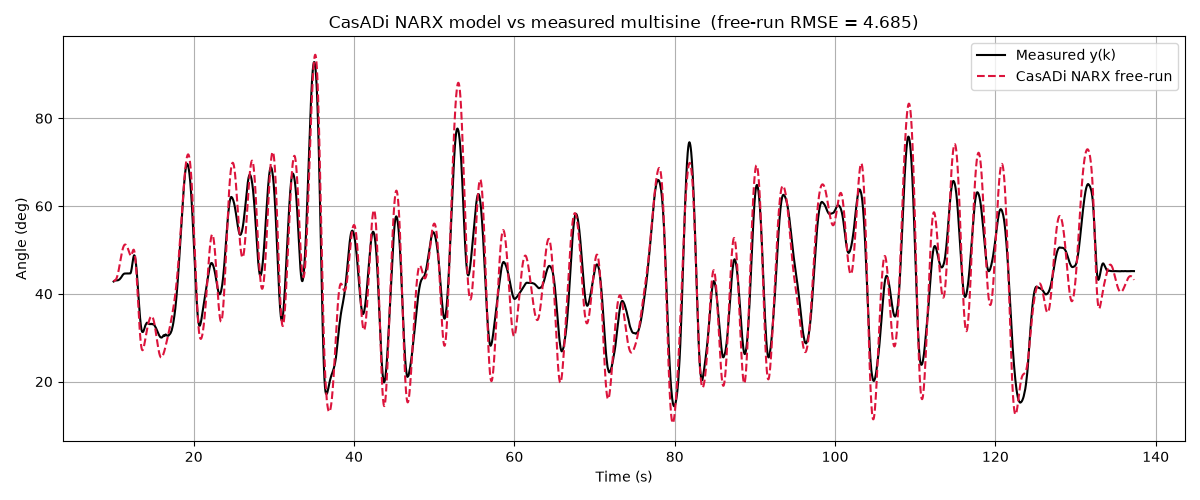
\includegraphics[width=\textwidth]{imagens/narx_freerun.png}
    \caption{Modelo NARX (implementado no CasADi) versus multisseno medido: simulação livre, RMSE = 4,685\graus{}.}
    \label{fig:narx_fr}
\end{figure}

\begin{itemize}
    \item \textbf{RMSE em simulação livre = 4,685\graus{}} no multisseno de validação. É um bom resultado para um modelo de 10 termos simulado livremente por cerca de 130\,s.
    \item \textbf{Fase muito bem capturada}: picos e vales do modelo ocorrem nos mesmos instantes que os medidos.
    \item \textbf{Amplitude superestimada nos extremos}: o modelo ultrapassa picos e vales (ex.: em 53\,s, 88\graus{} contra 78\graus{} medidos; em 105\,s, 12\graus{} contra 20\graus{}). Isso indica que \textbf{o modelo é menos amortecido que a planta real}, o que é coerente com o polo próximo de 1.
    \item \textbf{Implicação para o controle}: o MPC foi projetado para uma planta "mais viva" do que a real. Na bancada, a planta mais amortecida e com atrito tende a \textbf{atrasar e atenuar} a resposta, como se observa na validação~3 (Seção~\ref{sec:real}).
    \item \textbf{Faixa de validade}: o treino cobriu apenas 45\graus{} e 60\graus{}, mas as referências de validação do controle chegam a cerca de 105\graus{}. Nessa faixa o modelo está \textbf{extrapolando}, o que explica os erros em regime nos degraus altos.
\end{itemize}

\subsection{Observações sobre o script \texttt{narx.py}}
\begin{itemize}
    \item Há comentários desatualizados no script: "20--80\,s" (o corte real é de 10\,s/13\,s) e "últimos 5 segundos" (o código usa 13\,s). A questão é apenas cosmética.
    \item O relatório principal chama o NARX de "\textbf{modelo fenomenológico}". \atencao{Isso está incorreto}: o NARX polinomial é um modelo caixa-preta, orientado a dados. O correto é dizer que ele possui termos fisicamente interpretáveis.
\end{itemize}

%==========================================================
\section{Simulação em Python (NMPC com CasADi e rede neural)}
%==========================================================

\subsection{MPC nominal}

\begin{figure}[H]
    \centering
    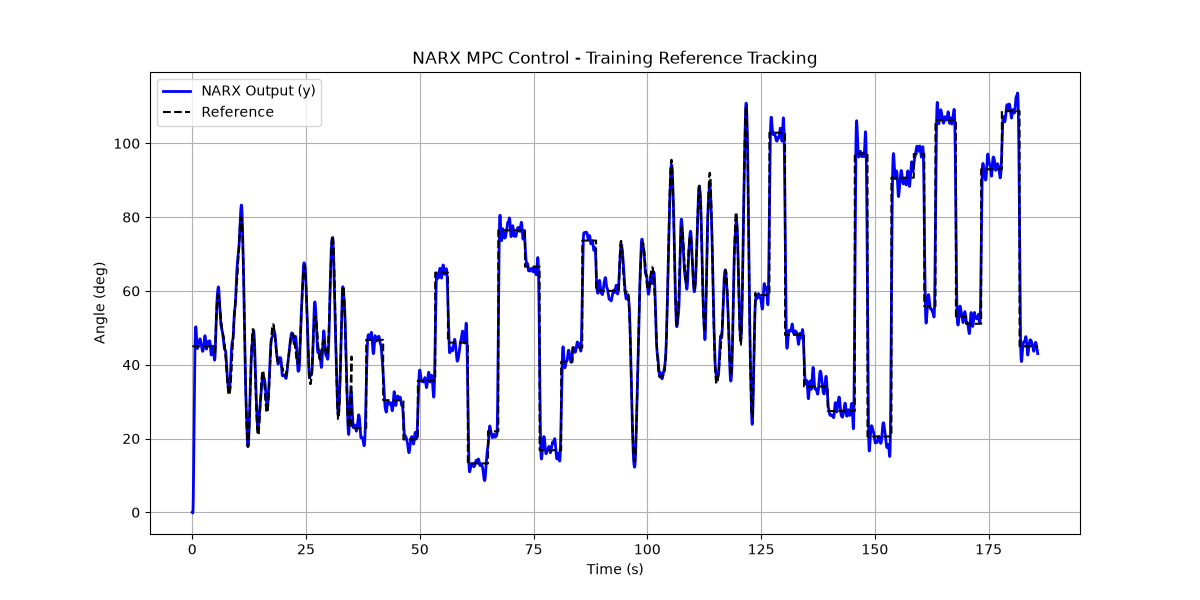
\includegraphics[width=0.9\textwidth]{imagens/mpc_treino.png}
    \caption{NMPC baseado no NARX rastreando a referência usada para gerar o \textit{dataset} de treino.}
    \label{fig:mpc_treino}
\end{figure}

\begin{itemize}
    \item A referência de treino combina um multisseno ($f_{max} = 0{,}5$\,Hz) com degraus aleatórios, totalizando 187\,s e cobrindo \textbf{de cerca de 12\graus{} a 110\graus{}}. É uma boa cobertura do domínio para gerar o \textit{dataset}.
    \item O rastreamento é quase perfeito porque \textbf{a planta simulada é o próprio modelo} (não há incerteza). O resultado serve como \textbf{limite superior de desempenho}, e não como prova de robustez.
    \item Aparecem pequenas oscilações nos patamares altos (90--110\graus{}, entre 145 e 185\,s). É a região em que o NARX extrapola e tem ganho local maior.
\end{itemize}

\subsection{Custo computacional}

\begin{figure}[H]
    \centering
    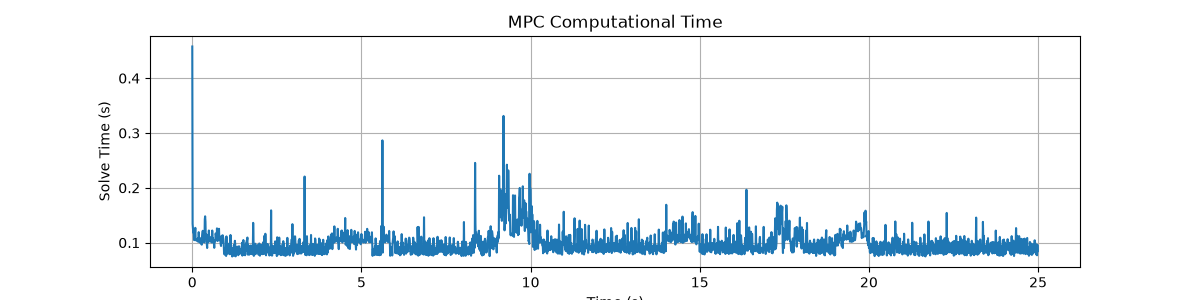
\includegraphics[width=\textwidth]{imagens/mpc_tempo.png}
    \caption{Tempo de solução do NMPC (CasADi) a cada passo de controle.}
    \label{fig:mpc_tempo}
\end{figure}

\begin{itemize}
    \item O tempo de solução típico é de \textbf{90--110\,ms}, com picos de \textbf{0,33--0,46\,s}: \textbf{de 10 a 45 vezes o período de amostragem} $T_s = 10$\,ms.
    \item \textbf{Este é o argumento central do trabalho}: o NMPC \textit{online} é inviável até em um PC e, portanto, ainda mais no STM32F446. Isso justifica aproximar a lei de controle por uma rede neural (MPC explícito aproximado).
    \item Os picos coincidem com transitórios da referência (cerca de 9--10\,s), quando o \textit{solver} precisa de mais iterações e as restrições ficam ativas.
\end{itemize}

\subsection{Treinamento da rede neural}

\begin{figure}[H]
    \centering
    \begin{minipage}{0.38\textwidth}
        \centering
        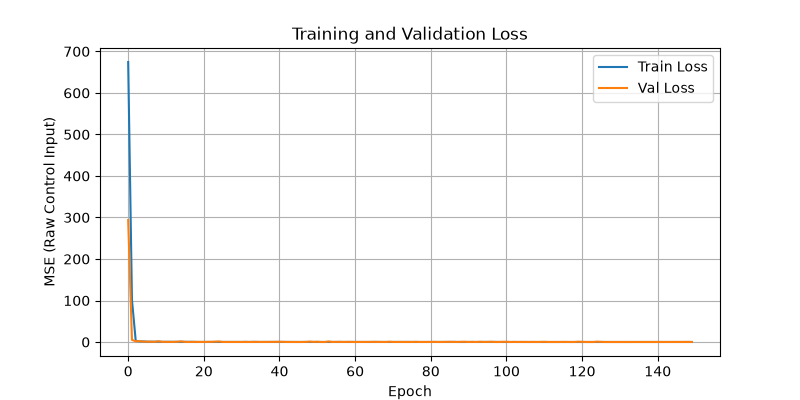
\includegraphics[width=\textwidth]{imagens/ann_loss.png}
    \end{minipage}\hfill
    \begin{minipage}{0.60\textwidth}
        \centering
        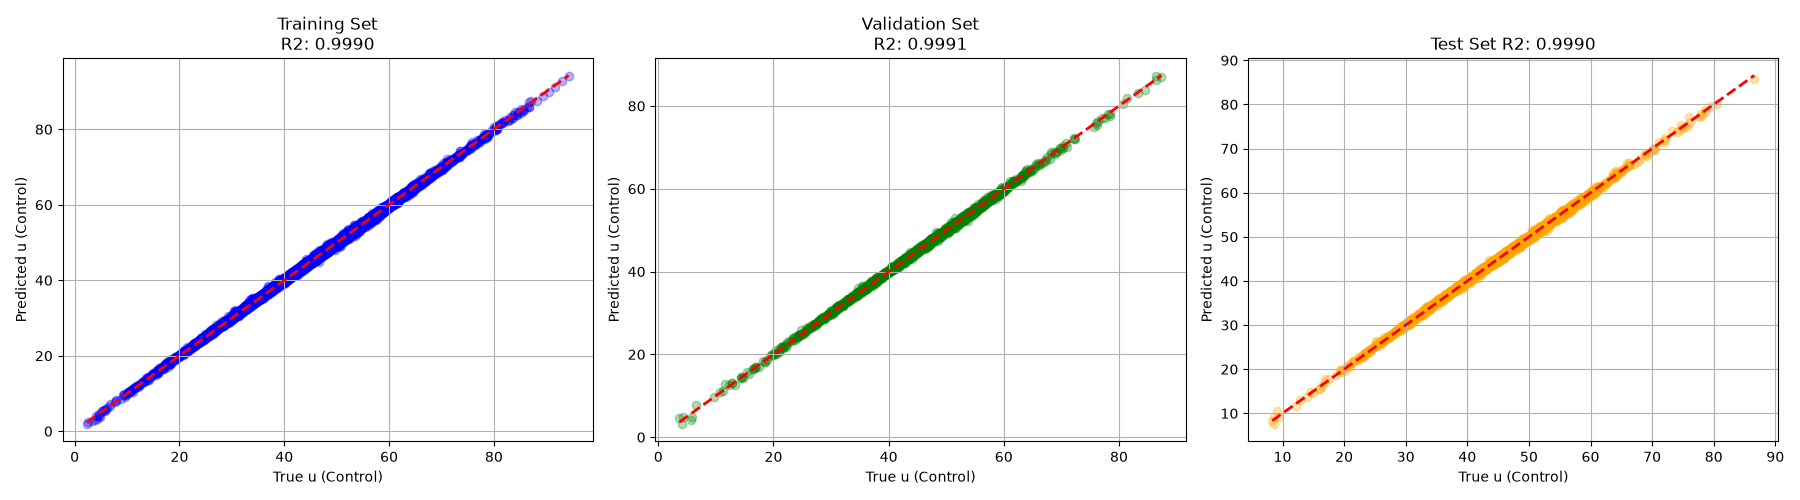
\includegraphics[width=\textwidth]{imagens/ann_r2.png}
    \end{minipage}
    \caption{Curvas de perda (MSE) por época e dispersão $u$ predito $\times$ $u$ ótimo nos conjuntos de treino, validação e teste.}
    \label{fig:ann}
\end{figure}

\begin{itemize}
    \item A perda converge em \textbf{menos de 5 épocas}, e as curvas de treino e validação ficam sobrepostas, ou seja, \textbf{não há sobreajuste}.
    \item $\mathbf{R^2 = 0{,}999}$ nos conjuntos de treino, validação e teste. Há leve dispersão apenas para $u < 10\,\%$, região pouco amostrada.
    \item \textbf{Ressalva importante}: um $R^2$ alto na imitação passo a passo de $u$ \textbf{não garante} bom desempenho em malha fechada, porque pequenos erros podem se acumular ao longo do tempo. Por isso a validação em malha fechada, apresentada a seguir, é indispensável.
\end{itemize}

\subsection{Rede neural em malha fechada com o NARX}

O protocolo de todos os ensaios é: \textbf{PID (0--5\,s) $\rightarrow$ rede neural (5--70\,s) $\rightarrow$ PID (70--75\,s)}.

\begin{figure}[H]
    \centering
    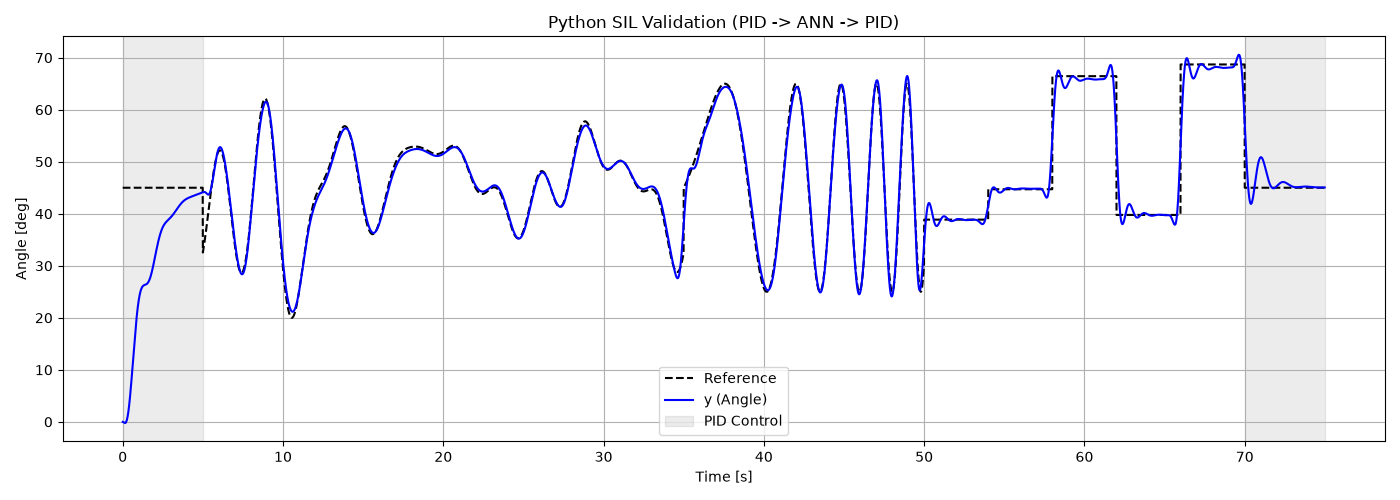
\includegraphics[width=\textwidth]{imagens/py_val1.png}\\[2pt]
    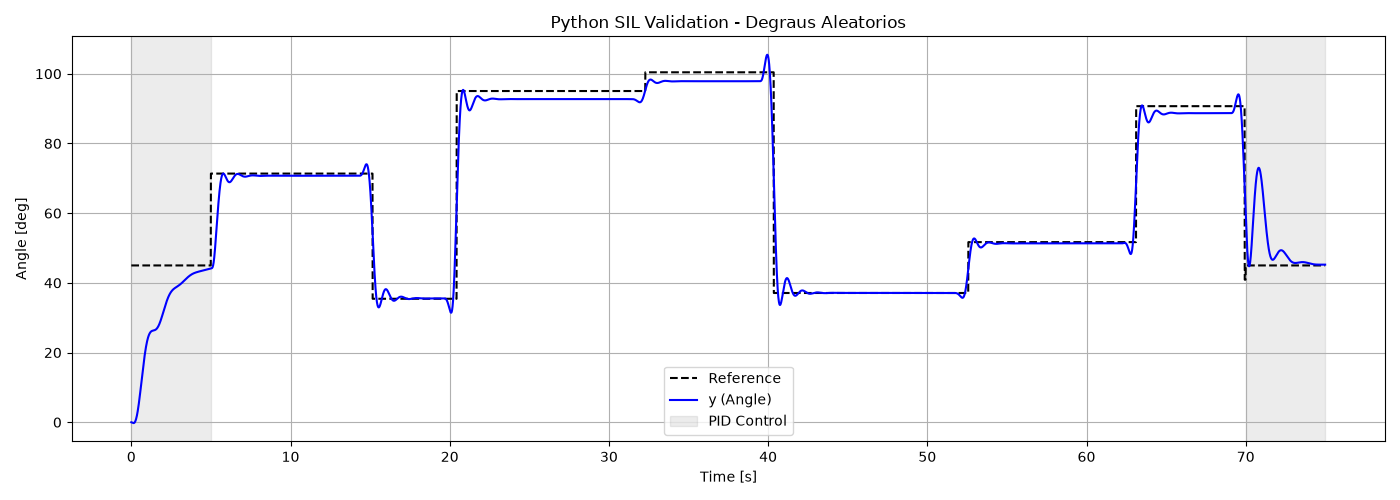
\includegraphics[width=\textwidth]{imagens/py_val2.png}\\[2pt]
    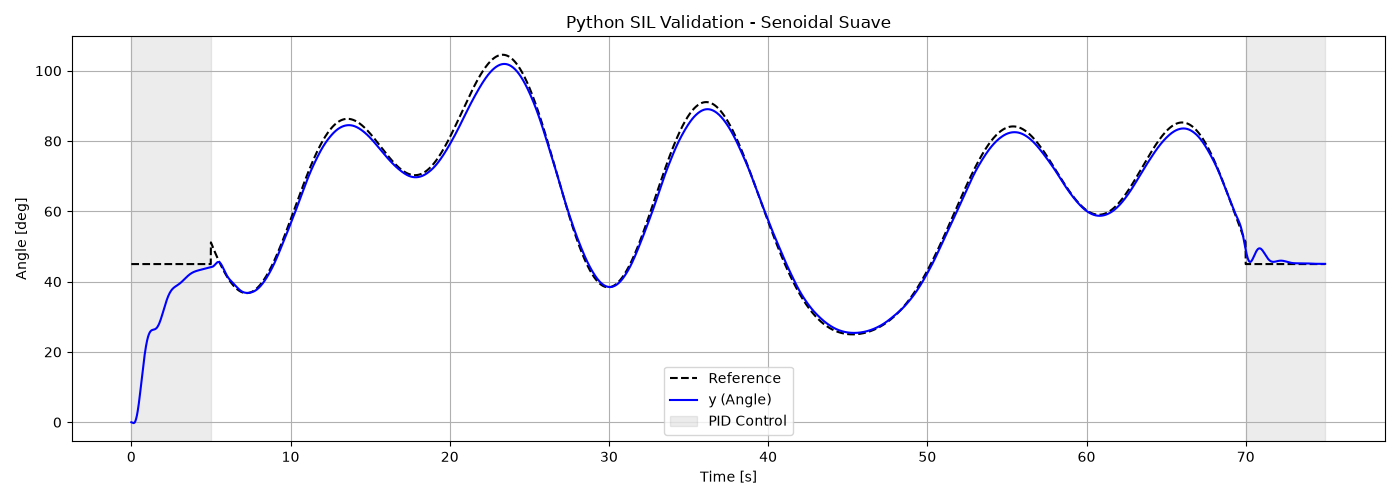
\includegraphics[width=\textwidth]{imagens/py_val3.png}
    \caption{Simulação em Python da rede neural em malha fechada com o NARX: validação~1 (multisseno + degraus), validação~2 (degraus aleatórios) e validação~3 (senoidal suave).}
    \label{fig:py}
\end{figure}

\begin{itemize}
    \item \textbf{Validação 1 (multisseno + degraus), RMSE 1,56\graus{}}: rastreamento excelente, inclusive no \textit{chirp} entre 40 e 50\,s, com pequeno sobressinal nos degraus (cerca de 2--3\graus{}).
    \item \textbf{Validação 2 (degraus aleatórios), RMSE 4,31\graus{}}:
    \begin{itemize}
        \item \textbf{Erro em regime nos degraus altos}: 95\graus{} $\rightarrow$ 93\graus{}; 100,5\graus{} $\rightarrow$ 98\graus{}; 91\graus{} $\rightarrow$ 89\graus{}. O erro aparece mesmo com planta igual ao modelo, porque \textbf{a rede neural não tem ação integral} e esses pontos estão perto da borda do \textit{dataset}.
        \item O RMSE é dominado pelos próprios degraus (erro inevitável no instante da troca de referência), por isso não é diretamente comparável ao das validações 1 e 3.
    \end{itemize}
    \item \textbf{Validação 3 (senoidal suave), RMSE 1,37\graus{}}: atenuação de cerca de 2\graus{} nos picos (86\graus{} contra 84\graus{}; 104\graus{} contra 102\graus{}), comportamento típico de um MPC que penaliza variações de controle ($\Delta u$).
    \item \textbf{Antecipação dos degraus}: $u$ e $y$ começam a se mover \textit{antes} da troca de referência (ex.: em 14,5\,s e 39,5\,s na validação~2). Isso é o \textbf{\textit{preview} da referência} do MPC, aprendido pela rede neural, e deve ser destacado como característica positiva do MPC.
    \item \textbf{Transição da rede neural para o PID em 70\,s}: aparece um salto na resposta (na validação~2 em Python, o ângulo vai de 45\graus{} a 73\graus{}). A transferência não é suave (\textit{bumpless}).
\end{itemize}

%==========================================================
\section{SIL no STM32 (rede neural embarcada em C com planta NARX)}
%==========================================================

\begin{figure}[H]
    \centering
    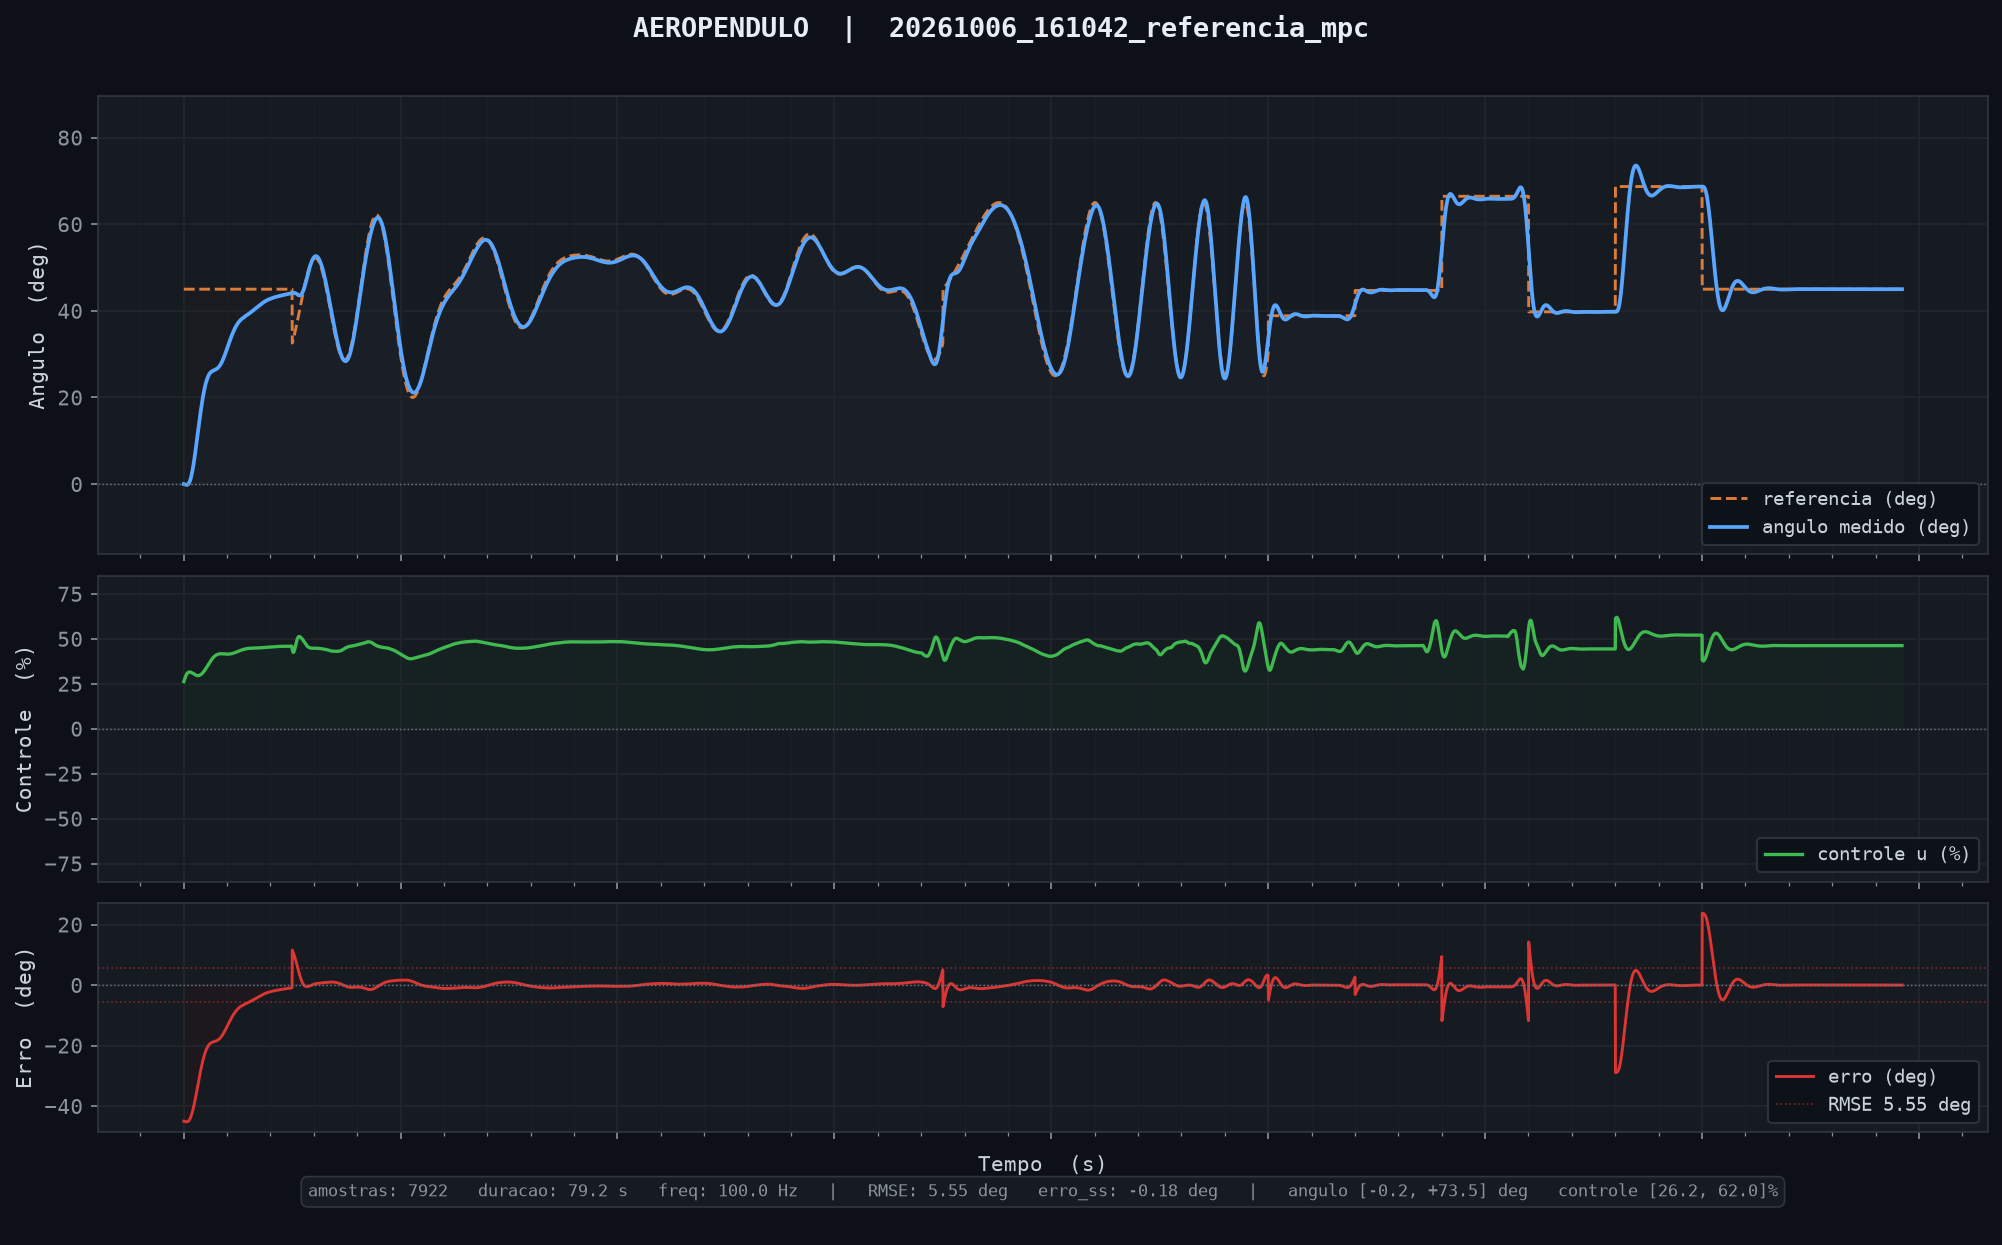
\includegraphics[width=0.85\textwidth]{imagens/sil_val1.png}
    \caption{SIL no STM32, validação~1 (multisseno + degraus). O RMSE indicado no gráfico inclui a fase de partida com o PID.}
    \label{fig:sil1}
\end{figure}

\begin{figure}[H]
    \centering
    \begin{minipage}{0.49\textwidth}
        \centering
        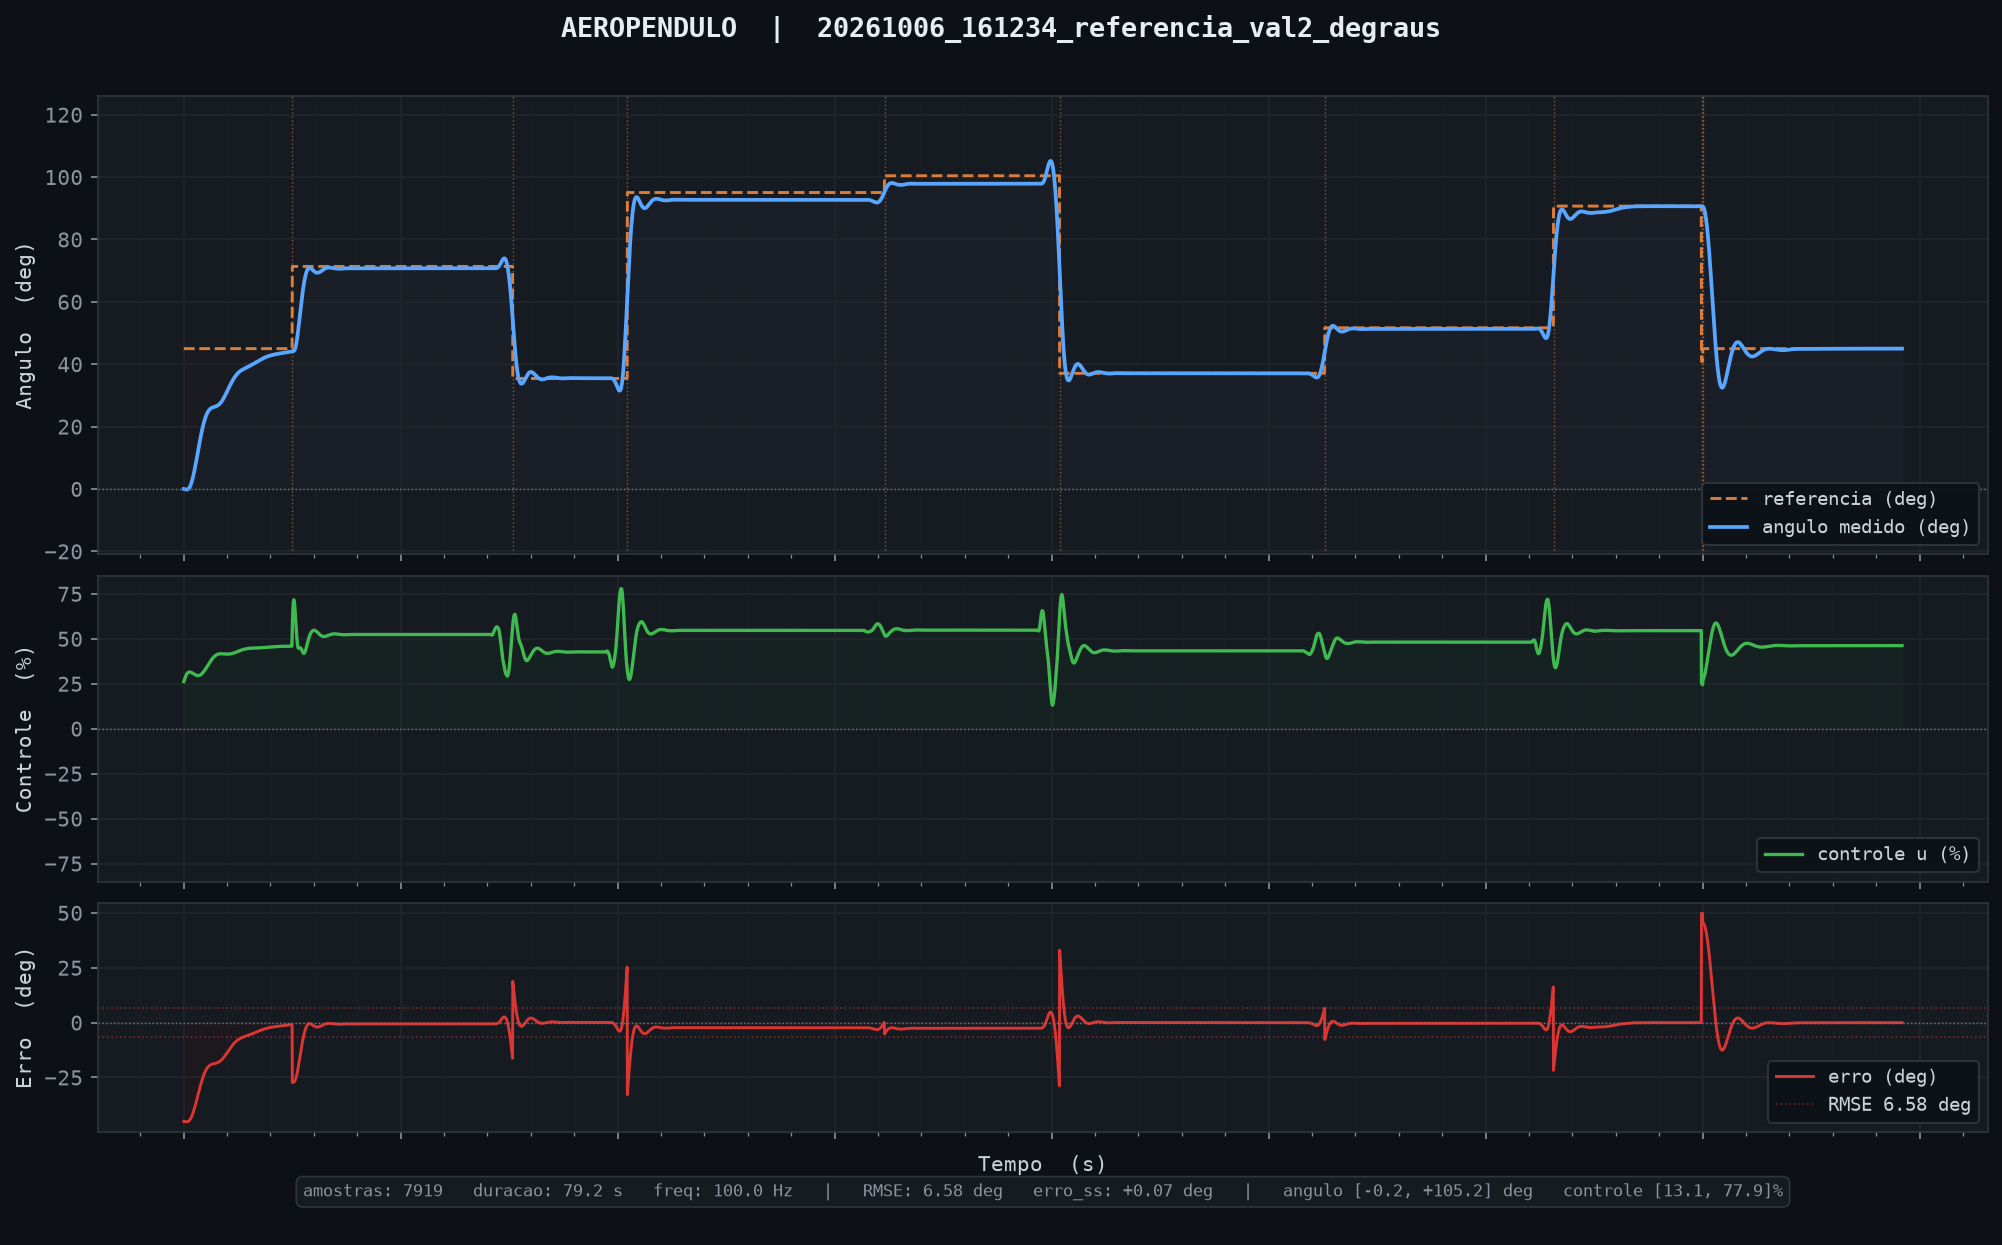
\includegraphics[width=\textwidth]{imagens/sil_val2.png}
    \end{minipage}\hfill
    \begin{minipage}{0.49\textwidth}
        \centering
        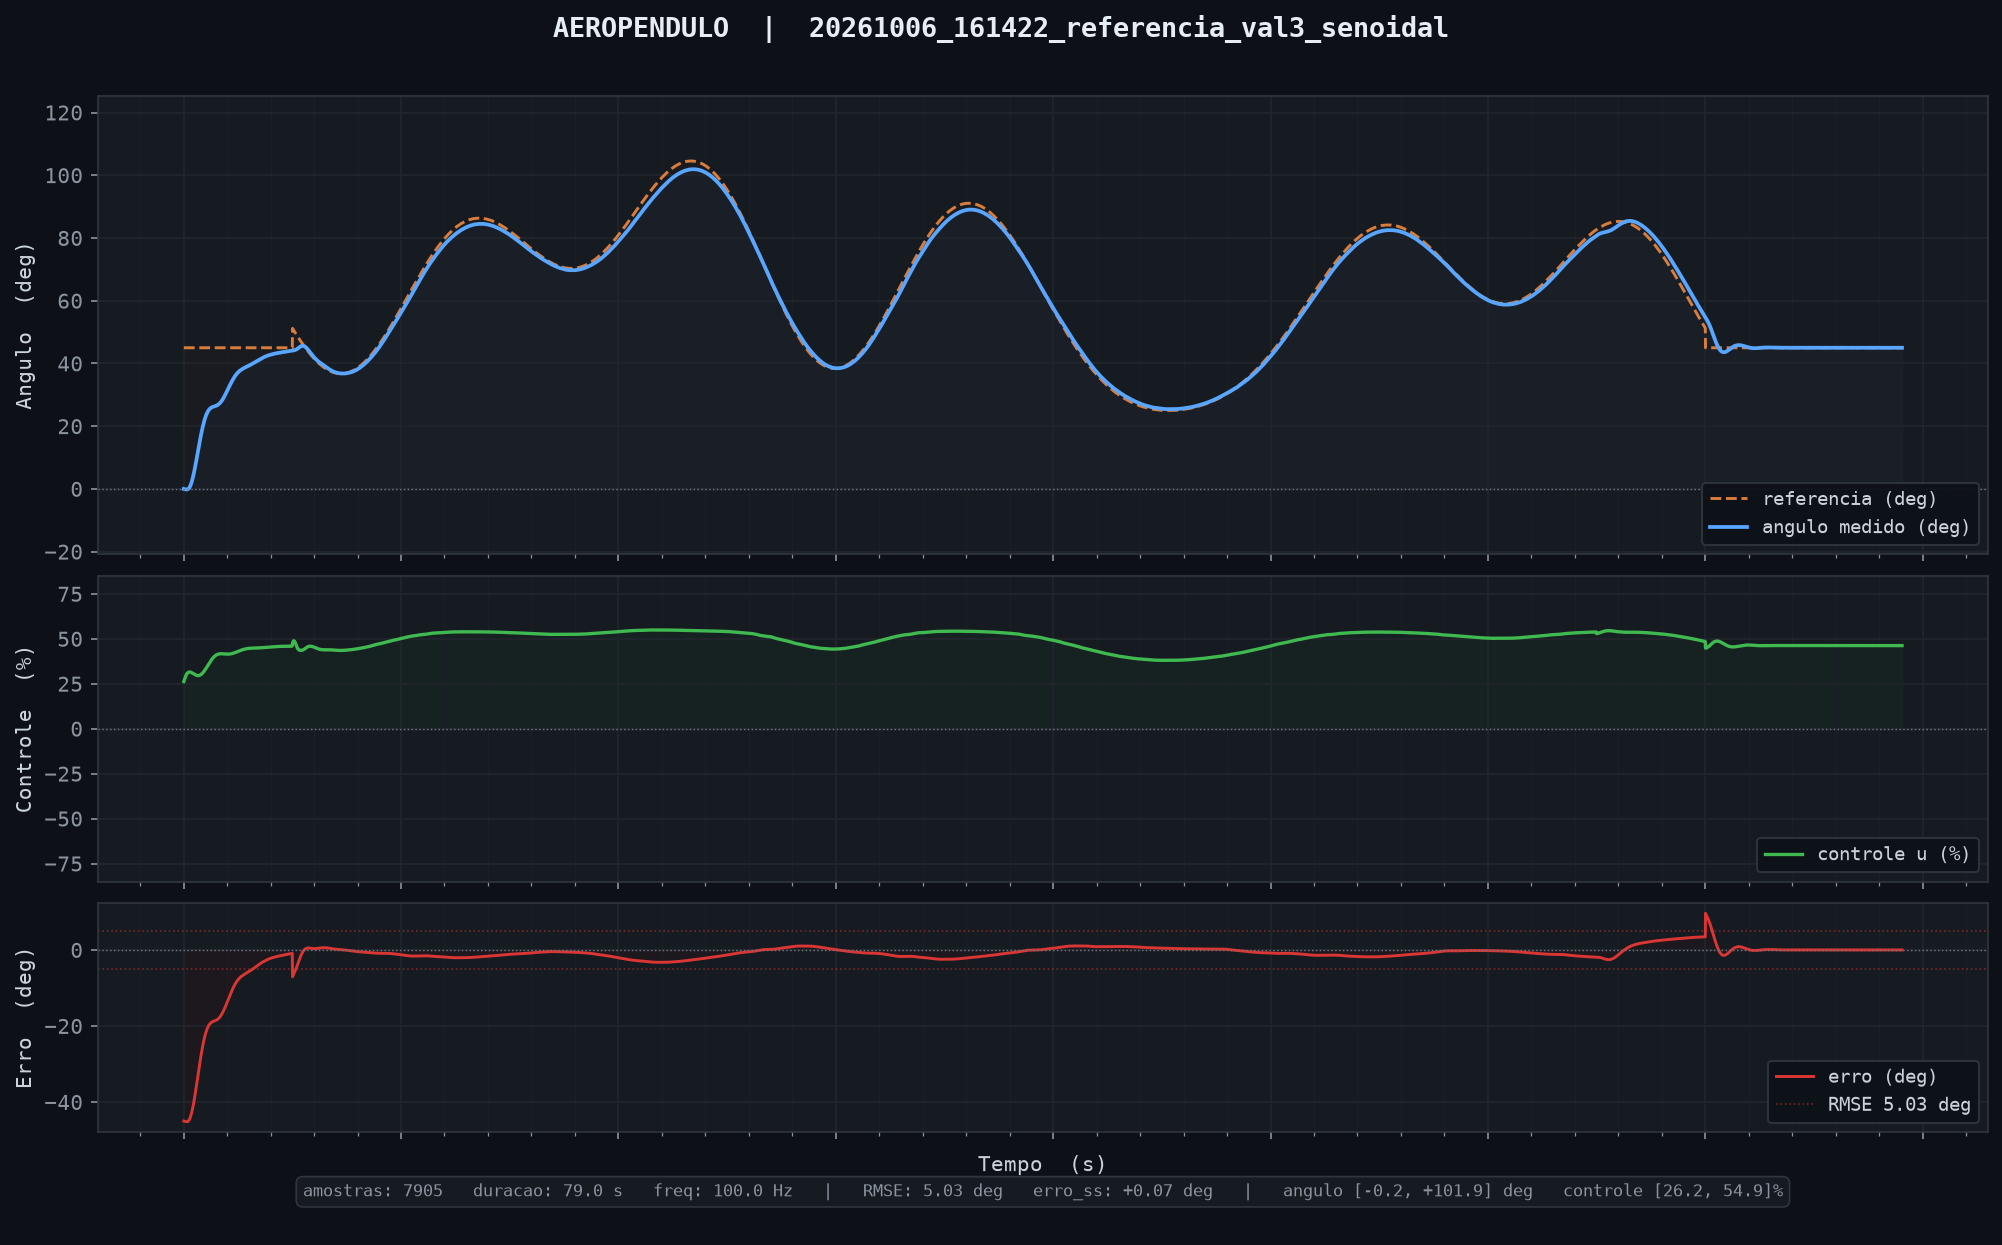
\includegraphics[width=\textwidth]{imagens/sil_val3.png}
    \end{minipage}
    \caption{SIL no STM32: validação~2 (esquerda) e validação~3 (direita).}
    \label{fig:sil23}
\end{figure}

\begin{itemize}
    \item \textbf{As curvas do STM32 e do Python ficam praticamente sobrepostas} durante a janela da rede neural, nos três testes (Figuras~\ref{fig:val1_cmp}--\ref{fig:val3_cmp}). Isso confirma:
    \begin{itemize}
        \item a \textbf{fidelidade numérica} da exportação dos pesos (\texttt{ann\_weights.h}) e da inferência em C (\texttt{float32} no STM32 contra \texttt{float64} no PyTorch);
        \item que a inferência cabe no período de 10\,ms: não houve perda de amostras (7919 a 7922 amostras em 79,2\,s, ou seja, cerca de 100\,Hz).
    \end{itemize}
    \item \textbf{Os erros em regime da validação~2 (93\graus{} contra 95\graus{}) aparecem iguais no SIL}. Isso \textbf{mostra que eles vêm da rede neural/modelo, e não do hardware}: as causas ficam isoladas.
    \item \textbf{Divergências entre Python e STM32 que merecem investigação}:
    \begin{itemize}
        \item Na validação~1 (65,5--70\,s) e na validação~2 (69--70\,s), o \textbf{Python antecipa} a troca de referência ($u$ oscila entre 35 e 63\,\%), mas o \textbf{STM32 não}. Hipótese: perto do fim da janela, o vetor de referência futura (horizonte de \textit{preview}) é montado de forma diferente nos dois ambientes (por exemplo, \textit{buffer} truncado ou preenchido com o último valor).
        \item Depois dos 70\,s (PID), a resposta do STM32 é mais suave que a do Python.
    \end{itemize}
    \item \atencao{Inconsistência de RMSE}: o gráfico do SIL na validação~1 mostra \textbf{5,55\graus{}}, mas a tabela do relatório informa \textbf{2,85\graus{}}. O valor do gráfico inclui a partida com o PID (erro inicial de $-45^\circ$). Na validação~2 ocorre o mesmo: 6,58\graus{} no gráfico e 4,63\graus{} na tabela.
    \begin{itemize}
        \item \textbf{Recomendação}: calcular o RMSE \textbf{somente na janela da rede neural (5--70\,s)}, igual para os três ambientes, e deixar isso explícito no texto.
        \item Também chama atenção a diferença na validação~1 entre Python (1,56\graus{}) e SIL (2,85\graus{}) com curvas visualmente sobrepostas. Isso sugere \textbf{janela de cálculo ou alinhamento temporal diferente} entre os arquivos CSV.
    \end{itemize}
\end{itemize}

%==========================================================
\section{Bancada real (aeropêndulo)}\label{sec:real}
%==========================================================

\subsection{Validação 1: multisseno + degraus (RMSE 3,26\graus{} na tabela; 5,50\graus{} no gráfico)}

\begin{figure}[H]
    \centering
    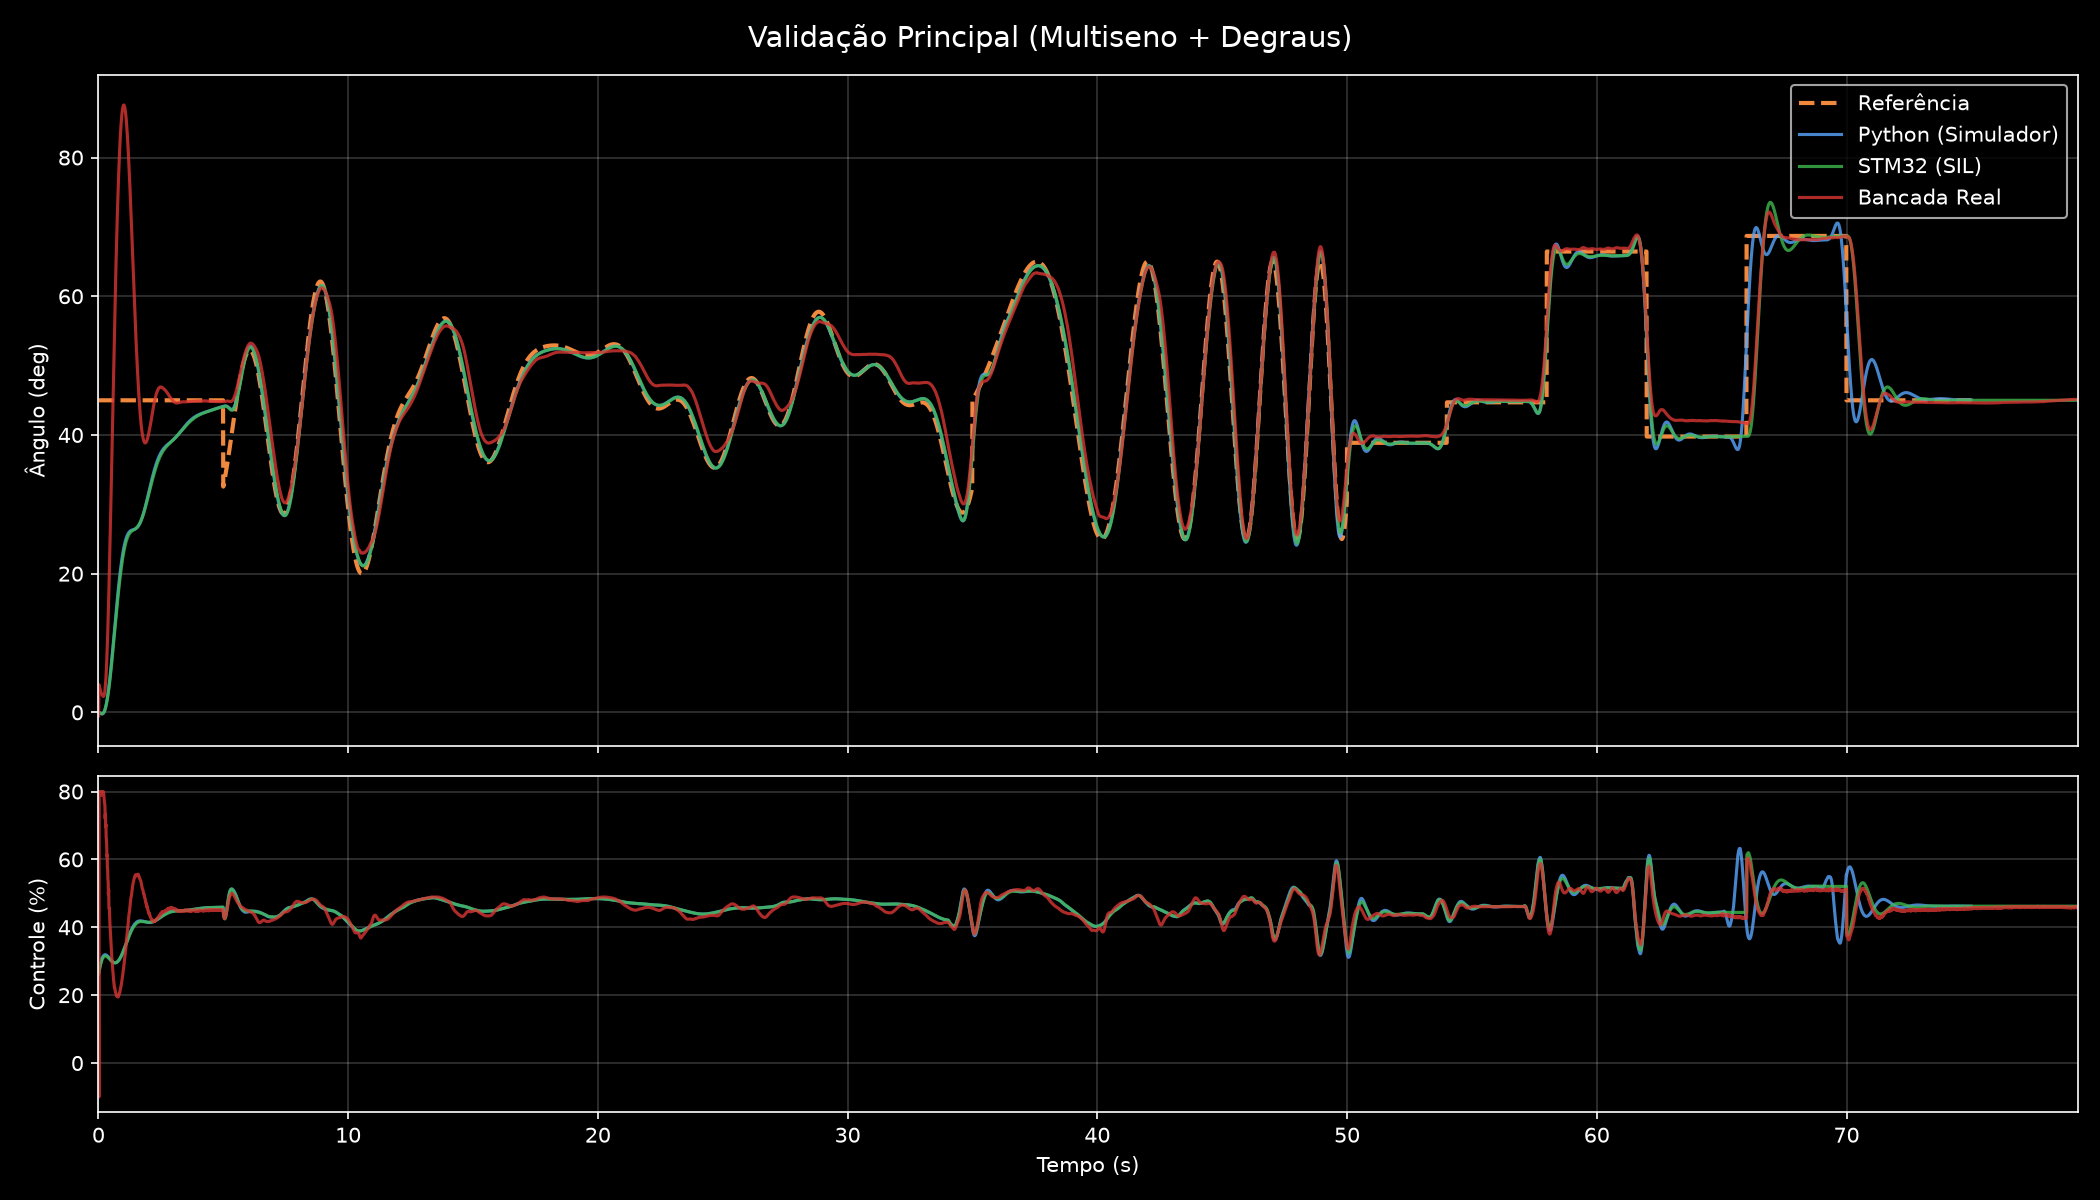
\includegraphics[width=\textwidth]{imagens/comparacao_plot_0.png}
    \caption{Validação~1: comparação entre Python, SIL (STM32) e bancada real.}
    \label{fig:val1_cmp}
\end{figure}

\begin{itemize}
    \item \textbf{Partida problemática}: sobressinal até \textbf{87,6\graus{}} em cerca de 1\,s, com $u$ saturando em \textbf{80\,\%} e depois em $-10\,\%$. No SIL a partida é suave ($u$ mínimo de 26\,\%). Isso indica diferença no PID ou nas condições iniciais da bancada (integrador, armação do ESC). \textbf{Não é um problema da rede neural}, mas é um ponto de segurança a mencionar.
    \item \textbf{Trecho rápido (\textit{chirp}, 40--50\,s)}: a bancada acompanha muito bem, com amplitude e fase quase iguais às da simulação. É o resultado mais expressivo do ensaio.
    \item \textbf{Trechos lentos (28--34\,s)}: a bancada fica \textbf{3 a 5\graus{} acima} da referência quando esta desce. Isso indica \textbf{atrito/histerese no mancal} e o amortecimento subestimado pelo NARX.
    \item \textbf{Erros em regime}: entre 62 e 66\,s, a bancada fica em 42\graus{} para uma referência de 40\graus{} (+2\graus{}). Sem ação integral, qualquer diferença de ganho estático entre modelo e planta vira erro permanente.
\end{itemize}

\subsection{Validação 2: degraus aleatórios (RMSE 4,77\graus{} na tabela; 6,79\graus{} no gráfico)}

\begin{figure}[H]
    \centering
    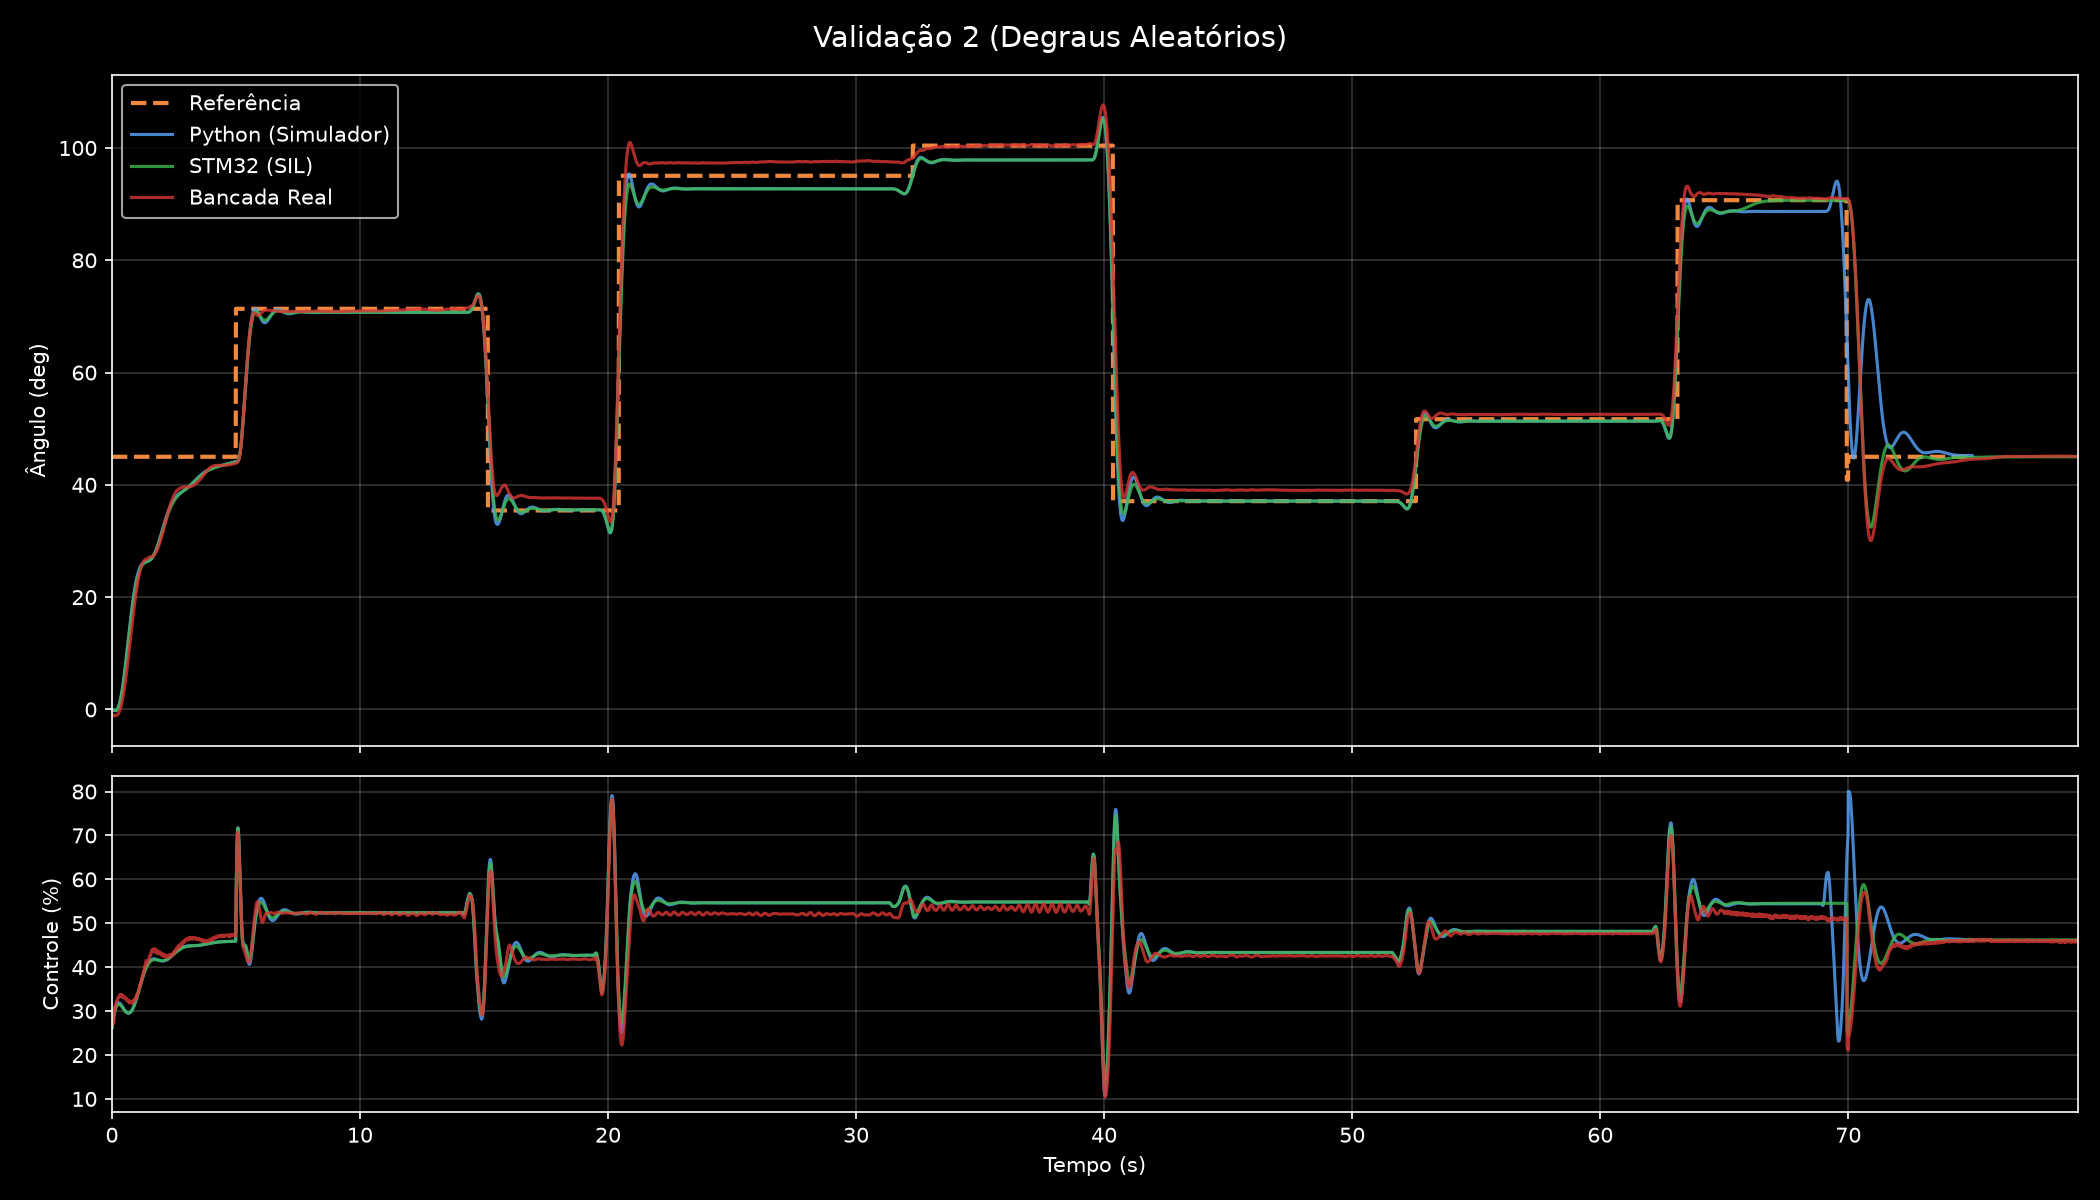
\includegraphics[width=\textwidth]{imagens/comparacao_plot_1.png}
    \caption{Validação~2: comparação entre Python, SIL (STM32) e bancada real.}
    \label{fig:val2_cmp}
\end{figure}

\begin{itemize}
    \item \textbf{Erro em regime com sinal oposto ao da simulação}: para 95\graus{}, a bancada vai a \textbf{97,5\graus{}}, enquanto o SIL fica em 93\graus{}; para 37\graus{}, a bancada vai a \textbf{39\graus{}}, enquanto o SIL fica em 37\graus{}. A planta real tem \textbf{ganho maior} que o NARX nessas regiões, que estão fora da faixa de treino (45--60\graus{}).
    \item \textbf{Oscilação no controle} nos patamares altos (32--40\,s, $u \approx 53\,\%$): um pequeno ciclo-limite, causado pelo ruído da IMU combinado ao ganho elevado da rede neural na região de extrapolação.
    \item Os transitórios (sobressinal e antecipação) são \textbf{muito parecidos} com os do SIL, o que indica que a dinâmica rápida foi bem modelada.
    \item \textbf{Menor degradação relativa} entre os três testes (4,77/4,31 $\approx$ \textbf{1,1}), porque o RMSE é dominado pelo erro inevitável no instante de cada degrau.
\end{itemize}

\subsection{Validação 3: senoidal suave (RMSE 3,01\graus{} na tabela; 5,82\graus{} no gráfico)}

\begin{figure}[H]
    \centering
    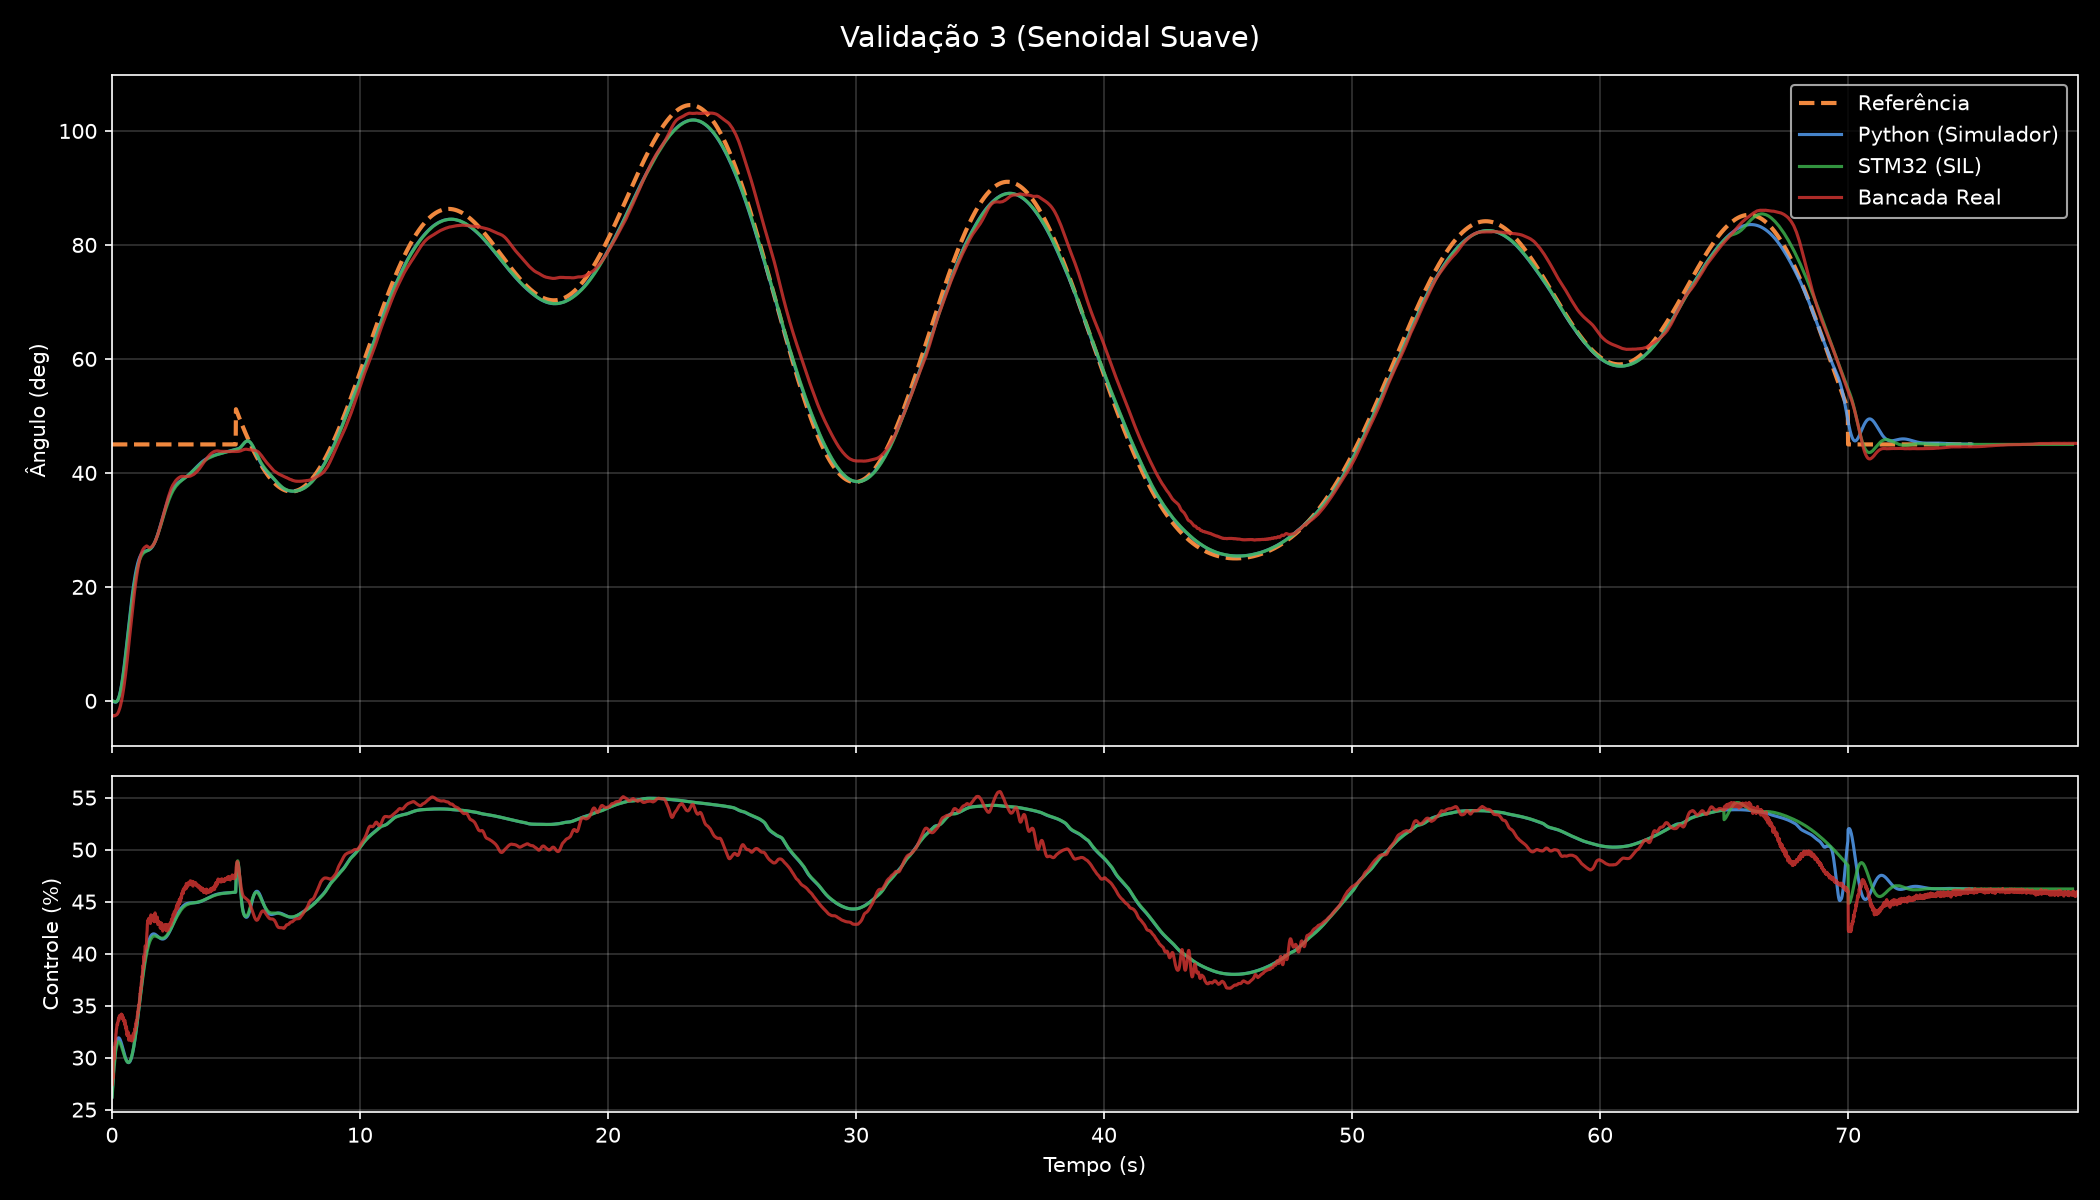
\includegraphics[width=\textwidth]{imagens/comparacao_plot_2.png}
    \caption{Validação~3: comparação entre Python, SIL (STM32) e bancada real.}
    \label{fig:val3_cmp}
\end{figure}

\begin{itemize}
    \item \textbf{Atraso de fase} da bancada de cerca de 0,5--1\,s em relação à simulação, mais visível nas descidas (25--28\,s e 38--42\,s).
    \item \textbf{Vales atenuados}: 42\graus{} contra 38\graus{} (em 30\,s) e 28\graus{} contra 25\graus{} (em 45\,s). Os \textbf{trechos planos} em 15\,s, 37\,s e 57\,s mostram o pêndulo "parando" quando a velocidade troca de sinal: é a \textbf{assinatura clássica de atrito estático (\textit{stick-slip})}, que o NARX não captura.
    \item O controle real \textbf{se afasta do simulado} (até cerca de 3\,\%) justamente nesses trechos, porque a realimentação está compensando a diferença entre modelo e planta. Também aparece ruído de alta frequência em $u$, vindo da IMU.
    \item \atencao{Maior degradação relativa: 3,01/1,37 $\approx$ 2,2.} Isso \textbf{contradiz o texto atual do relatório}, que apresenta este ensaio como o de maior proximidade entre bancada e simulador.
\end{itemize}

\subsection{Quadro-resumo da degradação}

\begin{table}[H]
    \centering
    \caption{RMSE (\graus{}) e degradação relativa ao simulador Python.}
    \label{tab:degradacao}
    \begin{tabular}{@{}lccccc@{}}
        \toprule
        \textbf{Teste} & \textbf{Python} & \textbf{SIL} & \textbf{Bancada} & \textbf{SIL/Python} & \textbf{Bancada/Python} \\ \midrule
        Val.~1 (multisseno + degraus) & 1,56 & 2,85 & 3,26 & 1,8$\times$  & 2,1$\times$ \\
        Val.~2 (degraus aleatórios)   & 4,31 & 4,63 & 4,77 & 1,07$\times$ & \textbf{1,1$\times$} \\
        Val.~3 (senoidal suave)       & 1,37 & 1,50 & 3,01 & 1,1$\times$  & \textbf{2,2$\times$} \\ \bottomrule
    \end{tabular}
\end{table}

%==========================================================
\section{Pontos a corrigir ou reforçar no relatório principal}
%==========================================================
\begin{itemize}
    \item \textbf{"Modelo fenomenológico NARX"}: trocar por "modelo caixa-preta NARX polinomial com termos fisicamente interpretáveis".
    \item \textbf{Validação 3}: em termos relativos, não é o ensaio de maior proximidade entre bancada e simulador. A diferença deve ser atribuída ao \textbf{atrito no mancal} e ao \textbf{amortecimento subestimado} pelo modelo.
    \item \textbf{Padronizar a janela do RMSE} (5--70\,s) e explicar a diferença em relação aos valores dos gráficos individuais.
    \item \textbf{"No-windup"} (validação~2): a rede neural não tem integrador, então o termo não se aplica. É melhor escrever "ausência de saturação prolongada".
    \item \textbf{"Quantizado" e "$<10$\,ms"}: só manter se houver medição (tempo de inferência por ciclo, uso de Flash/RAM). Caso contrário, escrever "pesos em \texttt{float32} exportados para C".
    \item \textbf{ReLU e EMPC afim por partes}: no MPC \textit{linear}, a lei de controle é afim por partes, mas aqui o MPC é \textbf{não-linear}. É melhor dizer que a rede neural "aproxima" a lei de controle, em vez de "compatível".
    \item \textbf{Acrescentar}: a análise do ganho estático, o argumento do tempo de solução do NMPC e a interpretação física dos termos $u^2$ como empuxo.
\end{itemize}

%==========================================================
\section{Melhorias sugeridas (trabalhos futuros)}
%==========================================================
\begin{itemize}
    \item Incluir dados de treino do NARX em \textbf{mais pontos de operação} (30\graus{}, 75\graus{}, 90\graus{} ou mais) para eliminar a extrapolação.
    \item Adicionar \textbf{ação integral}: erro integrado como entrada da rede neural, ou um MPC \textit{offset-free} com estimador de perturbação, para eliminar os erros em regime de cerca de 2\graus{}.
    \item Modelar o \textbf{atrito} (termos dependentes do sinal da velocidade) ou partir para uma identificação caixa-cinza (\textit{greybox}).
    \item Tornar a transição entre PID e rede neural \textbf{suave} (\textit{bumpless}).
    \item Verificar a construção do \textbf{\textit{preview} da referência} no STM32 perto do fim da janela da rede neural.
\end{itemize}

\end{document}
